\documentclass{abrice}

\title{Comp 491: Capstone Proposal}
\author{Anthony Brice\protect\\\medskip David Claveau, PhD.}
\date{\today\protect\\ \bigskip Aggregate Metadata Browsing Over HTTP}

\usepackage[style=nature,natbib=true,backend=biber]{biblatex}
\addbibresource{proposal.bib}

\usepackage{flowchart}
\usetikzlibrary{arrows}
\usetikzlibrary{positioning}

\usepackage{pgfgantt}

\setcounter{secnumdepth}{2}

\begin{document}
\maketitle

\section{Introduction}

Many music players, especially web-based, give the user very little control
over the ways in which one can sort and filter music. Miller columns have come
to be the de facto standard for browsing and visualizing a music database, but
most players only give the user a few columns tied to particular metadata, like
the common Album Artist--Album sort. Those that do allow the user to define an
arbitrary number of columns on arbitrary metadata are exclusively native
applications which expect their database and physical music files to be located
on the same device. This capstone proposes a client--server application with a
centralized music database communicating with many web-based clients allowing a
rich set of sorting and filtering capabilities.

\section{Background}

The problem of digital asset management, especially as it pertains to large
music libraries, is not a new one. Many metadata browsers exist but vary widely
in the control they give to their users over the ability to sort and
filter. Apple's iTunes for example, easily the most ubiquitous media player,
allows the user to sort by year but not filter.

Musicbee, a popular third-party media player that serves as the inspiration for
this proposal, provides the user with up to 6 Miller columns with which one can
sort and filter the database~\cite{musicbee}. Unfortunately it is also a
closed-source application native to Windows only.

Quod Libet, an open-source and cross-platform media player, takes the novel
approach of foregoing a traditional database in favor of creating serialized set
of Python objects with which to query~\cite{quodlibet}. This choice may be too
clever for its own good, as filters over as few as three metadata frames tend to
require quite large amounts of RAM for large databases (on the order of 1GB for
60K music files). Like the previous examples Quod Libet is also a native desktop
application that expects its database and files to reside on the same physical
device.

Subsonic is a popular client--server media player and another inspiration for
this proposal~\cite{subsonic}. It offers an easy-to-use web interface connected
to a server but only provides a few canned sorts, such as Album Artist--Album
and randomized Genre playlists.

\section{Requirements}

As shown in Fig.~\ref{fig:arch}, the program will have the common
database/application/client architecture. It will provide a Web interface to an
online music database such that a client will have the ability to create and
stream dynamic playlists with ease. Any source written in service of
implementation will be licensed under version 3 of the GNU General Public
License.

\begin{figure}
  \label{fig:arch}
  \centering
  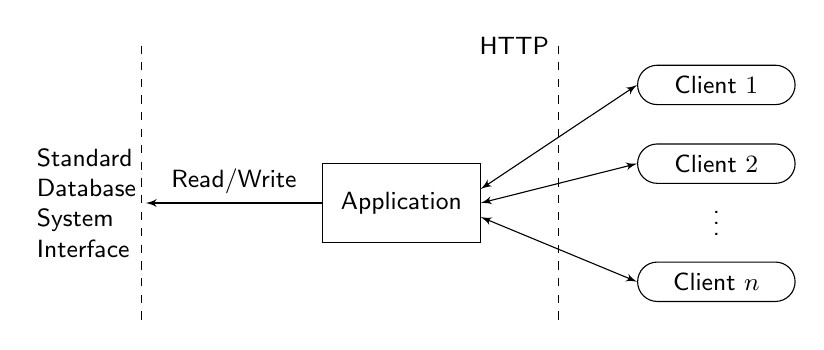
\begin{tikzpicture}[>=latex',font={\sffamily \small}]
    \def\smbwd{2cm}

    \node (database) at (-4, 0) [align=left] {Standard\\Database\\System\\Interface};

    \node (application) at (0,0) [draw, process,
    minimum width=\smbwd,
    minimum height=1cm] {Application};

    \node (client1) at (4,1.5) [draw, terminal,
    minimum width=\smbwd,
    minimum height=0.5cm] {Client $1$};

    \node (client2) at (4,0.5) [draw, terminal, minimum width=\smbwd, minimum
    height=0.5cm] {Client $2$};

    \node (elip) at (4,-0.15) {\vdots};

    \node (clientn) at (4,-1) [draw, terminal, minimum width=\smbwd, minimum
    height=0.5cm] {Client $n$};

    \draw [dashed] (-3.3,2) -- (-3.3,-1.5);
    \draw [dashed] (2,2) node[left] {HTTP} -- (2,-1.5);

    \draw[->] (application) -- node[above] {Read/Write} (database);
    \draw[<->] (application.10) -- (client1.west);
    \draw[<->] (application.east) -- (client2.west);
    \draw[<->] (application.350) -- (clientn.west);
  \end{tikzpicture}
  \caption{A block diagram describing the proposal's architecture.}
\end{figure}

\subsection{Functional Requirements}

\begin{enumerate}
\item Database
  \begin{enumerate}
  \item Provide a model of locally stored audio files.
  \item Include in each record all metadata frames defined in the associated
    file.
  \item Allow mutation of metadata during run time.
  \item Given a query, return a list of matching songs.
  \item Given a query and a specific metadata frame, return a list of values for
    that query and frame.
  \end{enumerate}

\item Application
  \begin{enumerate}
  \item Provide access to database for many clients.
  \item Host client interface.
  \item Manage authentication and authorization.
  \item Given a request to mutate a metadata frame of a song, ensure mutation is written
    both to database and file.
  \end{enumerate}

\item Client
  \begin{enumerate}
  \item Provide Miller column--browser interface to database.
  \item Manage display for viewports of varying size.
  \item Provide interface through which authorized users may update any metadata
    frame of a song or collection of songs.
  \item Stream selected playlist to connected audio device.
  \end{enumerate}
\end{enumerate}

\subsection{Performance Requirements}

\begin{enumerate}
\item Query performance must scale linearly as commodity hardware is added to
  database cluster.
\item Client--server round trip should take no longer then 2 seconds.
\end{enumerate}

\subsection{Cost}

\begin{enumerate}
\item Hardware for a server capable of handling a large personal music library
  (less than 100\,000 metadata records) should cost no more than 500~USD.
\item Any computer capable of running a web browser reasonably well, such as a 50~USD
  Raspberry Pi, should be capable of running the Web client.
\item I estimate development should take 15 hours per week over 12 weeks, or 180 hours.
\end{enumerate}

\section{Target Implementation}

The choice between a traditional SQL or document-oriented database is
non-obvious and will likely be determined through experimentation. A
document-oriented database such as MongoDB or Couchbase is desirable because of
their schema-less nature. I would like to avoid defining specific metadata
frames on which the client can sort since the ID3 specification allows the
creation of arbitrary frames. In addition these databases scale linearly on
commodity hardware, so there's little worry that a database could get too big to
function. Conversely, a document-oriented database may be undesirable because
the client does use the data in a very relational way, and I am unsure if they
can handle the queries I plan to support.

The application layer can be implemented in a number of existing web
frameworks. The nature of database-driven applications requires that the
application be tightly coupled to the database implementation, so it seems
simplest to me to pass that requirement onto the client, since having the
application define its own query language would not loosen the coupling but only
make the client tightly coupled to this application. As I see it, the
application layer should take take queries from the client in the database's
native language, pass them on to the client, and serve up the results. I will
experiment with allowing the application to keep cursors open to allow the
streaming of result sets in an asynchronous way (like how Gchat makes
asynchronous requests for one's chat history as one scrolls a chat window
upwards), but I do not know well this will scale since in the worst case it
requires an open database connection for every client.

\begin{marginfigure}[-6cm]
  \centering
  \includegraphics[height=7cm]{iphone1.png}
  \caption{Target GUI on small screen. The right menu icon allows the user to
    choose the metadata frame for which values are listed.}
  \label{fig:phone1}
\end{marginfigure}

The client will be served in standard HTML5/CSS/ECMAScript. It will be a
single-page application making heavy use of AJAX requests to deliver content.  I
would like to use a new functional-reactive DSL called Elm, which provides a
clean, Haskell-like syntax for defining such applications~\cite{czaplicki}. I
believe the modularity inherent to its pure and immutable design and the
performance benefits from its abstract ``virtual DOM'' (i.e., scene graph)
implementation will be quite useful to my front-end.

The GUI will gracefully scale to different-sized viewports, presenting Miller
columns of values for a particular metadata frame. A selected value will filter
the possible values of the next column, finally presenting the user with a list
of songs matching the selected frame values. (See Figs.~\ref{fig:phone1}
and~\ref{fig:browser1}.)

\begin{figure}
  \centering
  \includegraphics[height=7cm]{browser1.png}
  \label{fig:browser1}
  \caption{Target GUI on large viewport. The combobox at the top of each column
    allows the user to select a metadata frame.}
\end{figure}

\section{Project Plan}

\begin{figure}
  \centering
  \begin{ganttchart}[
    vgrid,
    title label font={\sffamily \small},
    bar label font={\sffamily \small},
    milestone label font={\sffamily \small \itshape\/}
    ]{1}{15}
    \gantttitle{Spring 2016}{15} \\
    \gantttitlelist{1,...,15}{1} \\
    \ganttbar{Dev. DB}{1}{3} \\
    \ganttlinkedbar{Dev. App. Layer}{2}{10} \\
    \ganttmilestone{Feature Complete}{7} \ganttnewline[]
    \ganttlinkedbar{Dev. Client}{4}{12} \\
    \ganttmilestone{Finalize API}{10} \ganttnewline[]
    \ganttlinkedbar{Presentation Prep.}{13}{15}
    \ganttlink{elem1}{elem2}
    \ganttlink{elem3}{elem4}
  \end{ganttchart}
  \caption{A Gantt chart describing the proposal's schedule.}
  \label{fig:gantt}
\end{figure}

\noindent
As shown in Fig.~\ref{fig:gantt}, I have broken the project into four distinct
phases with two milestones throughout. The phases divide into three development
phases---the database, application, and client components---and a final phase
for presentation preparations.

The database development phase should move quickly as it only entails a few,
relatively simple items: configuring and spinning up a database, writing a
program to handle importing a set of music files into the specific DBMS, and
writing documentation for configuration and the use of the import program.

Next started will be the application phase, and a few weeks into that I should
be ready to begin work on the client as well. Most work on both these layers
will be done in tandem since to offer the most useful API I expect to require a
clear understanding of the client's needs.

By week 7 I plan to have a feature-complete rough draft of my project. This may
seem early, but I expect the application to perform rather poorly at this point
and wish to leave a significant amount of time for tuning. By week 10 I expect
to be ready to finalize the application layer's API, spending weeks 11 and 12
polishing the client GUI\@. I leave 3 weeks at the end of the semester to
prepare for capstone presentations.

\printbibliography%

\end{document}
%%% Local Variables:
%%% mode: latex
%%% TeX-master: t
%%% End:
